\documentclass[tikz,border=6pt]{standalone}
\usepackage[T1]{fontenc}
\usepackage{newtxtext,newtxmath}
\usepackage{tikz}
\usetikzlibrary{arrows.meta,positioning,calc,backgrounds}

\definecolor{ink}{HTML}{172033}
\definecolor{greyLine}{HTML}{9CA3AF}
\definecolor{greyFill}{HTML}{F3F4F6}
\definecolor{qkC}{HTML}{B91C1C}
\definecolor{ovC}{HTML}{0B7285}
\definecolor{steerC}{HTML}{2E7D32}

\tikzset{
  >={Latex[length=2.4mm,width=1.7mm]},
  ctitle/.style={font=\bfseries,text=ink,align=center},
  note/.style={font=\scriptsize,text=steerC,align=center},
  rowlab/.style={font=\small\bfseries,align=center},
  poslab/.style={font=\scriptsize\bfseries,text=ink,align=center},
  feat/.style={draw,line width=0.8pt,rounded corners=2pt,minimum width=11mm,
    minimum height=11mm,font=\small\bfseries,text=ink,inner sep=1pt,align=center,fill=white},
  knob/.style={circle,draw=steerC,fill=steerC,text=white,font=\tiny\bfseries,
    inner sep=0.3pt,minimum size=4mm,line width=0.4pt},
  keytxt/.style={font=\scriptsize,text=ink,align=left,anchor=west},
  act/.style={font=\scriptsize,text=ink},
}

\begin{document}
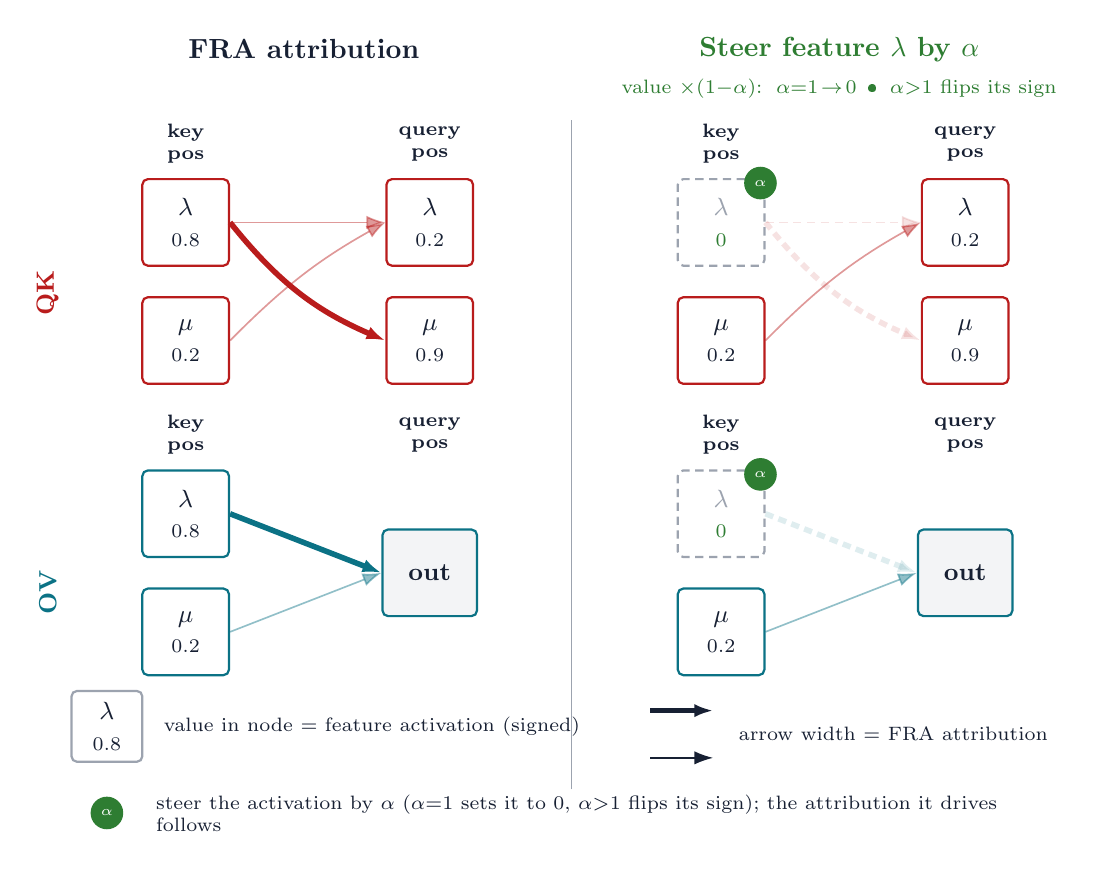
\begin{tikzpicture}[x=1mm,y=1mm]

\node[ctitle] at (34,98) {FRA attribution};
\node[ctitle,text=steerC] at (102,98) {Steer feature $\lambda$ by $\alpha$};
\node[note] at (102,93) {value $\times(1{-}\alpha)$:\, $\alpha{=}1\!\to\!0$ \,\textbullet\, $\alpha{>}1$ flips its sign};
\draw[greyLine,line width=0.4pt] (68,4) -- (68,89);

\node[rowlab,text=qkC,rotate=90] at (1.5,67) {QK};
\node[rowlab,text=ovC,rotate=90] at (1.5,29) {OV};

% ================= LEFT COLUMN =================
\node[poslab] at (19,86) {key\\pos}; \node[poslab] at (50,86) {query\\pos};
\node[feat,draw=qkC] (Lk1) at (19,76) {$\lambda$\\{\scriptsize$0.8$}};
\node[feat,draw=qkC] (Lk2) at (19,61) {$\mu$\\{\scriptsize$0.2$}};
\node[feat,draw=qkC] (Lq1) at (50,76) {$\lambda$\\{\scriptsize$0.2$}};
\node[feat,draw=qkC] (Lq2) at (50,61) {$\mu$\\{\scriptsize$0.9$}};
\draw[->,qkC,line width=0.6pt,opacity=0.45] (Lk1.east) -- (Lq1.west);
\draw[->,qkC,line width=0.6pt,opacity=0.45] (Lk2.east) to[bend left=8] (Lq1.west);
\draw[->,qkC,line width=2.0pt] (Lk1.east) to[bend right=14] (Lq2.west);
\node[poslab] at (19,49) {key\\pos}; \node[poslab] at (50,49) {query\\pos};
\node[feat,draw=ovC] (Lo1) at (19,39) {$\lambda$\\{\scriptsize$0.8$}};
\node[feat,draw=ovC] (Lo2) at (19,24) {$\mu$\\{\scriptsize$0.2$}};
\node[feat,draw=ovC,fill=greyFill,minimum width=12mm] (Lout) at (50,31.5) {out};
\draw[->,ovC,line width=2.0pt] (Lo1.east) -- (Lout.west);
\draw[->,ovC,line width=0.6pt,opacity=0.45] (Lo2.east) -- (Lout.west);

% ================= RIGHT COLUMN =================
\node[poslab] at (87,86) {key\\pos}; \node[poslab] at (118,86) {query\\pos};
\node[feat,draw=greyLine,densely dashed,text=greyLine] (Rk1) at (87,76) {$\lambda$\\{\scriptsize\textbf{\textcolor{steerC}{$0$}}}};
\node[knob] at ([xshift=5mm,yshift=5mm]Rk1.center) {$\alpha$};
\node[feat,draw=qkC] (Rk2) at (87,61) {$\mu$\\{\scriptsize$0.2$}};
\node[feat,draw=qkC] (Rq1) at (118,76) {$\lambda$\\{\scriptsize$0.2$}};
\node[feat,draw=qkC] (Rq2) at (118,61) {$\mu$\\{\scriptsize$0.9$}};
\draw[->,qkC,line width=0.6pt,densely dashed,opacity=0.13] (Rk1.east) -- (Rq1.west);
\draw[->,qkC,line width=0.6pt,opacity=0.45] (Rk2.east) to[bend left=8] (Rq1.west);
\draw[->,qkC,line width=2.0pt,densely dashed,opacity=0.13] (Rk1.east) to[bend right=14] (Rq2.west);
\node[poslab] at (87,49) {key\\pos}; \node[poslab] at (118,49) {query\\pos};
\node[feat,draw=greyLine,densely dashed,text=greyLine] (Ro1) at (87,39) {$\lambda$\\{\scriptsize\textbf{\textcolor{steerC}{$0$}}}};
\node[knob] at ([xshift=5mm,yshift=5mm]Ro1.center) {$\alpha$};
\node[feat,draw=ovC] (Ro2) at (87,24) {$\mu$\\{\scriptsize$0.2$}};
\node[feat,draw=ovC,fill=greyFill,minimum width=12mm] (Rout) at (118,31.5) {out};
\draw[->,ovC,line width=2.0pt,densely dashed,opacity=0.13] (Ro1.east) -- (Rout.west);
\draw[->,ovC,line width=0.6pt,opacity=0.45] (Ro2.east) -- (Rout.west);

% ================= LEGEND =================
\node[feat,draw=greyLine,minimum width=9mm,minimum height=9mm] at (9,12) {$\lambda$\\{\scriptsize$0.8$}};
\node[keytxt] at (15,12) {value in node $=$ feature activation (signed)};
\draw[->,ink,line width=2.0pt] (78,14) -- (86,14);
\draw[->,ink,line width=0.6pt] (78,8) -- (86,8);
\node[keytxt] at (88,11) {arrow width $=$ FRA attribution};
\node[knob] at (9,1) {$\alpha$};
\node[keytxt,text width=112mm] at (14,1) {steer the activation by $\alpha$ ($\alpha{=}1$ sets it to $0$, $\alpha{>}1$ flips its sign); the attribution it drives follows};

\end{tikzpicture}
\end{document}
